
\documentclass[a4paper]{article}

%%%%%%%%%%%%%%%%%%%%%%%%%%%%%%%%%% 
% Package for making LaTeX properly handle utf8 characters set and danish language rules
\usepackage[utf8]{inputenc}
\usepackage[danish]{babel}

%%%%%%%%%%%%%%%%%%%%%%%%%%%%%%%%%% 
% Package for changing to a nicer font 
\usepackage[T1]{fontenc}

%%%%%%%%%%%%%%%%%%%%%%%%%%%%%%%%%% 
% Package for conctroling the text area
\usepackage[margin=2.5cm]{geometry}

%%%%%%%%%%%%%%%%%%%%%%%%%%%%%%%%%% 
% Package for inserting clickable hyperlinks in pdf versions as produced by pdflatex
\usepackage{enumitem, hyperref}

%%%%%%%%%%%%%%%%%%%%%%%%%%%%%%%%%% 
% Package for including figures. TeX and thus LaTeX was developped before the existence of directory file-structures, but the graphicspath let's you add directories, that the \includegraphics will search.
\usepackage{graphicx}
\graphicspath{{figures/}}

%%%%%%%%%%%%%%%%%%%%%%%%%%%%%%%%%% 
% Package for typesetting programs. Listings does not support fsharp, but a little modification goes a long way
\usepackage{listings}
\usepackage{xcolor}
\usepackage{verbatim}
\usepackage{color}
\usepackage{textcomp}

\def\namedlabel#1#2{\begingroup
    #2%
    \def\@currentlabel{#2}%
    \phantomsection\label{#1}\endgroup
}

\definecolor{bluekeywords}{rgb}{0.13,0.13,1}
\definecolor{greencomments}{rgb}{0,0.5,0}
\definecolor{turqusnumbers}{rgb}{0.17,0.57,0.69}
\definecolor{redstrings}{rgb}{0.5,0,0}
\definecolor{lightgray}{RGB}{240, 240, 240}


\lstdefinelanguage{FSharp}
				{morekeywords={\#load, \#r, let, new, match, with, rec, open, module, namespace, type, of, member, and, for, in, do, begin, end, fun, function, try, mutable, if, then, else, List, Set, Sudoku, Seq, false, true, Assert, printfn, print, sprintf, when, ->, >, ::, printf, yield},
	keywordstyle=\color{bluekeywords},
	sensitive=false,
	morecomment=[l][\color{greencomments}]{///},
	morecomment=[l][\color{greencomments}]{//},
	morecomment=[s][\color{greencomments}]{{(*}{*)}},
	morestring=[b]",
	stringstyle=\color{redstrings},
	tabsize=2, % sets default tabsize to 2 spaces
	backgroundcolor=\color{lightgray}
}

\usepackage[table]{}
\usepackage{array}
\usepackage{algorithm}
\usepackage{caption}
\usepackage{float}
\usepackage{amsmath}
\usepackage{algorithm}
\usepackage[noend]{algpseudocode}
\usepackage{mathtools}
\usepackage{ragged2e}
\usepackage{caption}
\usepackage{amssymb}
\usepackage{listingsutf8}
\usepackage{newunicodechar}
%\newunicodechar{┌}{?}

% Site med mange eksempler - både kode og billeder
% http://www.texample.net/tikz/

%%% Tikz: pakke til at lave grafik
\usepackage{tikz}

%%% Tilføjer makroer der gør livet lettere for os
\usetikzlibrary{arrows, shapes, positioning}

%%% Pile
%%% http://www.texample.net/media/pgf/builds/pgfmanualCVS2012-11-04.pdf (afsnit 24)
\tikzset{
  aggr/.style={->, >=open diamond},
  inh/.style={->, >=open triangle 45}
} 

%%% Bokse
%%% http://www.texample.net/media/pgf/builds/pgfmanualCVS2012-11-04.pdf (afsnit 49)
\tikzset{
  class/.style={draw, rectangle}
}

\lstset{ %
  numbers=right,                    % where to put the line-numbers; possible values are (none, left, right)
  numbersep=5pt,                   % how far the line-numbers are from the code
  numberstyle=\small\color{bluekeywords}, % the style that is used for the line-numbers
  stepnumber=1,                    % the step between two line-numbers. If it's 1, each line will be numbered
  title=\lstname,                   % show the filename of files included with \lstinputlisting; also try caption instead of title
  showstringspaces=false,
  breaklines=true,
  captionpos=b,
  language=FSharp,
  texcl=true,
  inputencoding=utf8,
  extendedchars=true,
  mathescape=true,
  %escapeinside={(*}{*)},
  literate=
	{æ}{{\ae}}1
	{å}{{\aa}}1
	{ø}{{\o}}1
	{Æ}{{\AE}}1
	{Å}{{\AA}}1
	{Ø}{{\O}}1
	{ü}{{\"u}}1
	{├}{{?}}1
	{┐}{{?}}1
	{┌}{{?}}1
	{┘}{{?}}1
	{└}{{?}}1
	{╞}{{?}}1
	{╪}{{?}}1
	{╬}{{?}}1
	{┌}{{?}}1
	{┼}{{?}}1
}

\setlength\parindent{0pt}

\title{Simple Jack - Programmering og Problemløsning}
\author{Mads U. Svendsen, Anders F. Jørgensen, Nicolai L. Hargreave, Bo H. Thomsen}

\begin{document}
	\maketitle % Insert title etc.
        
  \tableofcontents

  \newpage

\section{Forord}
    
\section{Introduktion}
   \paragraph*{Sådan kompilerer du projektet\\}
    I \lstinline$/src$ mappen ligger der en Makefile og hvis man kører den, 
    kompileres \lstinline$game.exe$,
    begge filer kan findes i mappen \path{/src}.
    Kommandoen til at kompilerer er  \lstinline$make$ og kan den kan skrives i terminalen.

    Derudover kan man kompilerer projektet med dokumentation, ved at bruge kommandoen \lstinline$make withdocs$

    Tests findes i  mappen \path{/src}, i filen \lstinline$tests.fsx$,
    og kan kompileres med \lstinline$fsharpc$ og køres med \lstinline$mono$.

\newpage

\section{Problemformulering}
    
    \subsection{Kravspecifikation}

  \newpage

  \section{Problemanalyse og design}
    \subsection*{Struktur}
      I dette afsnit vil vi beskrive den strukturelle opbygning vi har overvejet i vores design.

      Vores design bygger op omkring fire kerne klasser,
      Game, Player, Hand og Card og en enumeration kaldet Suits - der huser de fire forskellige kulører.
      De forskellige klasser skal mimikke fysiske objekter og funktioner der forekommer i spillet.

      \subsubsection*{Game}
      Game gemmer Player objekttet for dealeren, en liste af Player objekter af de spillere der deltager
      og den nuværende stak der kan trækkes fra - denne stak er af typen Hand.
      Ved siden af det har den en funktion til at returnere antallet af spillere i spillet,
      det er i princippet bare en funktion der tager længden af players arrayen.
      Game indeholder også en funktion draw, der trækker et kort fra stack og ligger den ind i den valgte spillers hånd.

      Game objectets funktion er at holde styr på alt det nødvendige for spil logikken,
      så al datahåndtering til et spil foregår i dette objekt.

      \subsubsection*{Hand}
      Hand gemmer en array af Card objekter, og skal være et objekt der håndtere den funktion vores hånd har i et normalt kortspil.
      En hånd har en funktion der trækker et kort, altid det øverste(stak) denne har vi valgt at kalde \lstinline$drop$,
      den har en funktion der ligger et kort på stakken denne hedder \lstinline$draw$,
      så kan hele håndens kort erstattets, hånden skal kunne blandes og hånden skal kunne skrives ud som string.

      \subsubsection*{Player}
      En spiller/person skal have et navn(\lstinline$name$) i følge kravspecifikationen,
      vi bruger også Playerklassen til AI, så derfor har vi også en bool(\lstinline$AI$),
      \lstinline$index$ er array indexet for Playeren i Players arrayen, eller hvornår spilleren har tur,
      og hand er et Hand objekt der indeholder spillerens hånd.

      Ved siden af de properties har vi en \lstinline$score$ funktion der beregner spillens score,
      ved at gå gennem de kort der er i hånden.
      En \lstinline$isBusted$ der beregner om scoren er for høj og en \lstinline$scoreboard$,
      der laver en tekstrepræsentaiton af spillerens hånd og score.

      \subsubsection*{Card}
      Et spillekort har en kulør, se Sektionen \ref{sssec:suits}, og en værdi/index der repræsentere kortet,
      hvor 11 - 13 er (bonde, dame, konge) og numrene 2 - 10 har deres respektive værdi og et es har værdien 1.
      Denne værdi må ikke sammenblandes med den værdi kortet har i Blackjack,
      da alle billedkort har samme værdi - og derfor vil den værdi ikke være unik.
      Denne \lstinline$value$ sammenlædet med \lstinline$suit$ skaber en unik værdi,
      der kan bruges til at reprænsetere kortet når spillepladen vises.

      Udover suit og value, har kortet en funktion \lstinline$toString()$ der returnere en tekst repræsentation af kortet.
      \lstinputlisting[caption={Card's toString metode},label={lst:cardToString},firstline=18,lastline=32]{code/blackjack.fsx}

      \subsubsection*{Suits} \label{sssec:suits}
      En enumeration er, specielt i OOP, en god måde at repræsentere forskellige værdier for det sammen field, 
      når der kun er de mulige værdier for et field. I vores tilfælde, med \lstinline$Card.suit$,
      har vi kun de fire værdier og derfor ift validering, struktur m.m valgte vi at bruge en enumeration.


      \begin{figure}[H]
        \centering

        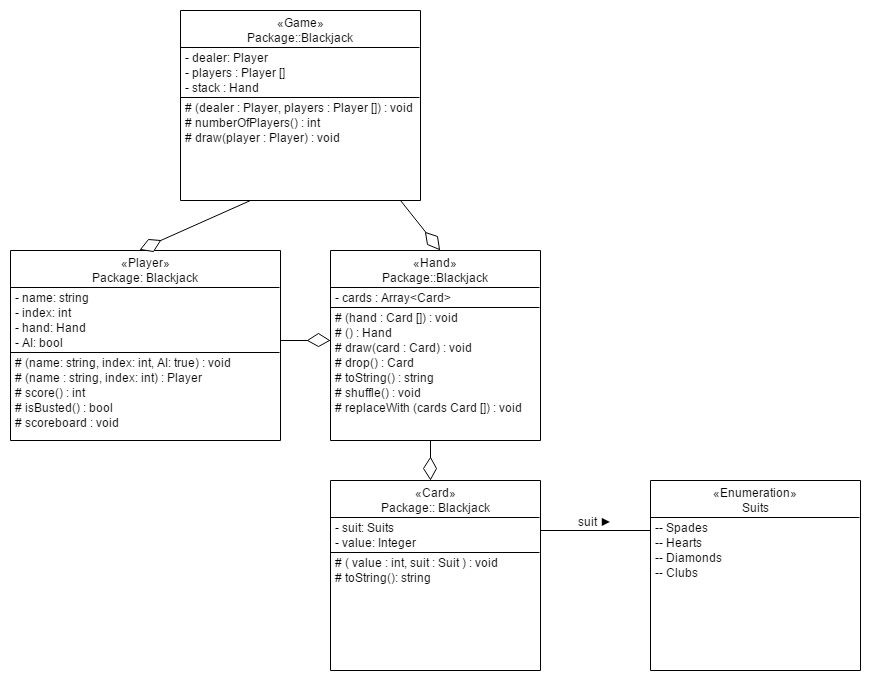
\includegraphics[width=520px]{figures/uml.png}

        \caption{UML diagram over vores klasse implementation}
        \label{fig:umlDiagram}
      \end{figure}

  \section{Programbeskrivelse}

  \section{Afprøvning} \label{sec:unitTest}

	\section{Diskussion og konlusion}
  
    \newpage
    \section{Bilag}
    
    \subsection{Brugervejledning}

    \subsection{Kildekode}
      \lstinputlisting[caption={Spilklasser},label={lst:blackjack}]{code/blackjack.fsx}
      \lstinputlisting[caption={Spillogikken},label={lst:game}]{code/game.fsx}
      \lstinputlisting[caption={Tests},label={lst:tests}]{../src/tests.fsx}
\end{document}